\documentclass{article}
\usepackage{tikz}
\begin{document}
\begin{center}
\Large{\textbf{Hierarchy of Linux distributions}}
\end{center}
\begin{figure}[h]
 \centering
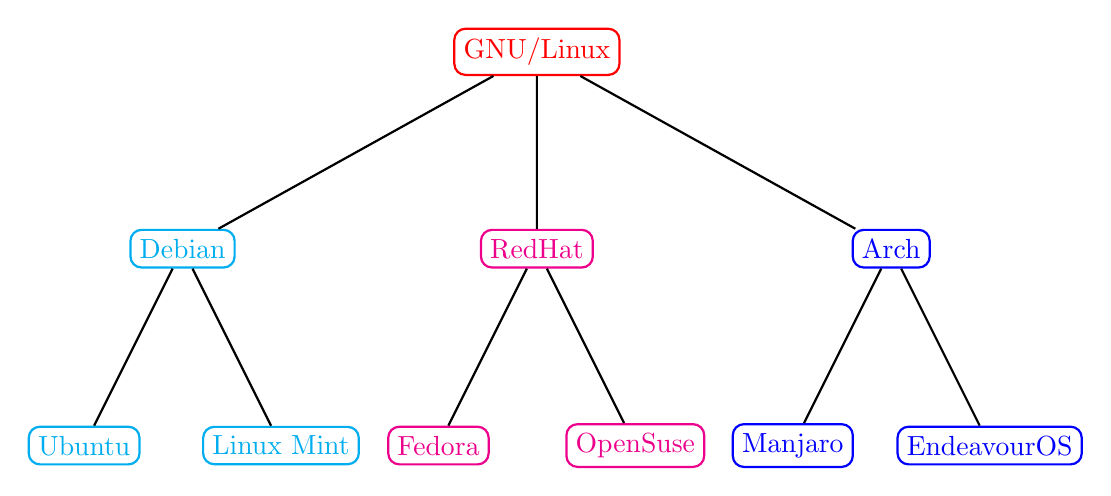
\begin{tikzpicture} [every node/.style = {shape=rectangle, rounded corners, draw, 
align=center}]
 \path [draw,thick,-]
 node (root)[red] {GNU/Linux}
 [sibling distance=45mm, level distance=25mm]
 child {node [cyan] {Debian} 
 [sibling distance=25mm, level distance=25mm]
 child { node [cyan] {Ubuntu} }
 child { node [cyan] {Linux Mint} }
% child { node {Elementary} }
 }
 child {node [magenta] {RedHat}
 [sibling distance=25mm, level distance=25mm]
 child { node [magenta] {Fedora} }
 child { node [magenta] {OpenSuse} } 
 }
 child {node [blue] {Arch}
[sibling distance=25mm, level distance=25mm] 
child { node [blue]{Manjaro} }
child { node [blue]{EndeavourOS} } 
 };
\end{tikzpicture}
\caption{GNU/Linux Operating System Family}
\end{figure}
\pagebreak
\begin{center}
\Large{\textbf{SUV Cars}}
\end{center}
\begin{figure}[h]
 \centering
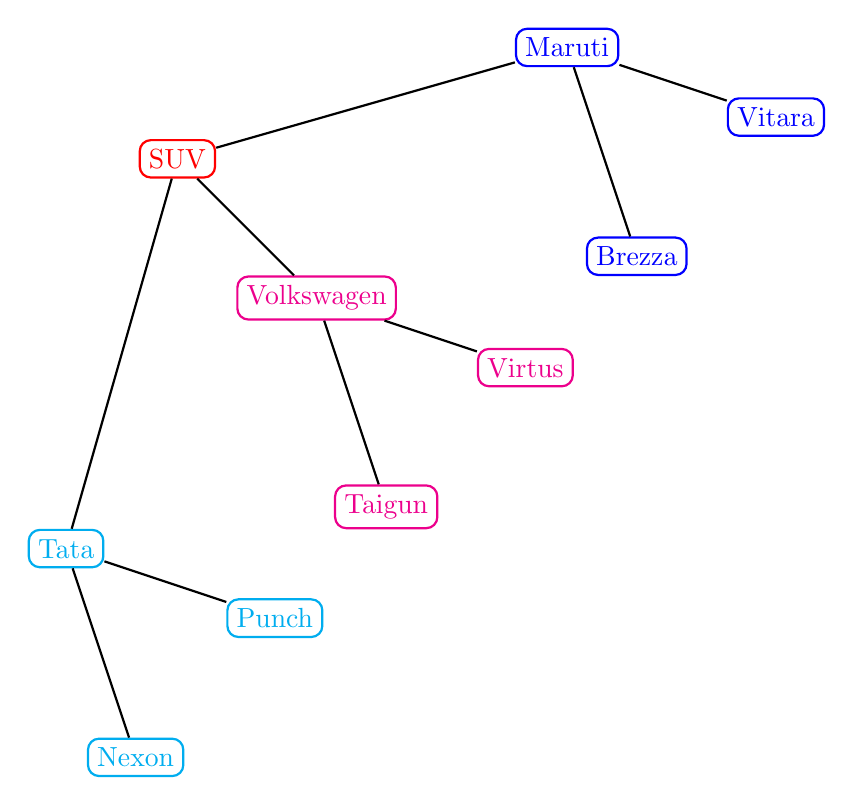
\begin{tikzpicture} [every node/.style = {shape=rectangle, rounded corners, draw, 
align=center}]
 \path [draw,thick,-]
 [grow=-45]
 node (root)[red] {SUV}
 [sibling distance=45mm, level distance=25mm]
 
 child {node [cyan] {Tata} 
 [sibling distance=25mm, level distance=25mm]
 child { node [cyan] {Nexon} }
 child { node [cyan] {Punch} }
% child { node {Elementary} }
 }
 child {node [magenta] {Volkswagen}
 [sibling distance=25mm, level distance=25mm]
 child { node [magenta] {Taigun} }
 child { node [magenta] {Virtus} } 
}
 child {node [blue] {Maruti}
[sibling distance=25mm, level distance=25mm] 
child { node [blue]{Brezza} }
child { node [blue]{Vitara} } 
 };
\end{tikzpicture}
\caption{Car Brands Hierarchy}
\end{figure}
\end{document}
